\chapter{Theory}
This chapter is going to explain theories behind the techniques used for this project. Each technique will be elaborated and how and when it is being used in the project will be explained.

%% Gustav suggestion: %%
%% This is ONLY theory and not implemenation (how we use it) %%

\section{Image Processing}
Image Processing can be described as an umbrella term. \citep{ip_book} writes that Image Processing comes from the general field of signal processing, and that it covers ways to segment objects of interest on a digital image. This is achieved using multiple steps. \citep{ip_book} describes them as follow. It should be noted, however, that the order of the steps sometimes change, and there might be more focus on some than others. That being said, this is a general framework that can be used as a good starting point:

\textbf{Image Acquisition}
Before anything can be processed, data needs to be captured, typically using a camera. This step is all about the setup, as well as the environment, setting, light, etc.

\textbf{Pre-processing}
Here the initial setup is completed, e.g. converting the image from color to grayscale.

\textbf{Segmentation}
To be able to work with a specific object, for instance a hand, it needs to be separated from the rest of the picture. This is done using segmentation where noise and background elements are removed, so only the object of interest is seen. Thresholding is often applied to make the object stand out, e.g. make the object appear white and the background black.

\textbf{Representation}
The object needs to be representative in an intuitive manner.

\textbf{Classification}
For the system to actually know that an object is a hand or not, it has to do some classification and compare the data to some knowledge or database. This can be done with template matching and BLOB classification.

Figure \eqref{fig:ip_framework} illustrates the framework used typically when working with Image Processing.

\begin{figure}[htbp]
\centering
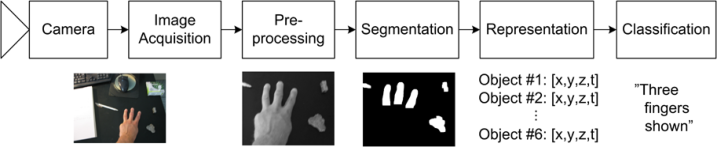
\includegraphics[width=1.00\textwidth]{Pictures/Theory/imageProcessing_steps.png}
\caption{Image Processing framework. - WE SHOULD MAKE OUR OWN PICTURE LATER ON!!!!!!!! - Gustav}
\label{fig:ip_framework}
\end{figure}

%% Maybe a little to blabla and too long sentences - Gustav %%
During this project a lot of image processing has been used. The different image processing techniques are used in a combination to display exactly what we want to output. Some techniques is being used to remove noise from the picture, so the important parts gets all the focus, while others are used for making the important parts more clear or making it possible to track specific parts of the output. \\
It is all these different techniques combined that makes it possible to get a functional product, but before you can use them, you will have to know how they work and how they can be included to your project. This section is going to explain the different techniques that are being used and also why and how they are being implemented in this project.

%% Could be a little more clear and short - Gustav %%
\section{Thresholding}
Threshold is one of the most fundamental operations in point processing \fixme{WHAT is point processing? - Gustav} and is used to make an input picture binary, i.e. either black (0) or white (255). Making an image binary means to show the image in only completely black and completely white pixel values. \\
This could be useful in programs where you need to find silhouettes - tracking a person for example - and smaller details are not as important. \\
To determine which pixels that should be completely black and which that should be completely white a threshold value is required. The threshold value can be compared to a gatekeeper that lets everyone who is 18 years old or older inside the club, but denies access to people that is 17 or younger. Using this analogy, pixels that are "old" (bright) enough are let in, while "younger" pixels (dark) are denied

Using the same analogy, somebody decided that the border between being too young and just old enough should be 18 years. This age could easily be something different, such as 17 or 24. The same is true with thresholding: you have to decide when pixels are "old" enough (bright). If they are too young (dark), they cannot get access.

In practice this means that pixels with values greater than a threshold is set to TRUE (or white), which typically is 255 when talking in bytes. On the other hand, if a pixel is less than the threshold value, it is set to FALSE (black) or 0. To sum this up the formula for making a threshold is shown in equation \ref{threshold}.
\begin{equation}
  \begin{aligned}
  	\text{if } f(x,y)\leq T \quad \text{then } g(x,y)=0 \\
  	\text{if } f(x,y)>T \quad \text{then } g(x,y)=255
	\label{threshold}  
  \end{aligned} 
\end{equation}
Where $T$ is the threshold value, $f(x,y)$ is the input pixel and $g(x,y)$ is the output pixel. 

When choosing the threshold value it is important to think about what the wanted output is. It differs  from image to image how effective thresholding is based on the difference between the object and the background. If the background and the object you want to find is very different in color, then it is easy to distinguish between them and choose an effective threshold value. However, if the object and background are very similar, then it becomes harder to do choose a threshold value, since you will have to chose between losing some information from the wanted object in order to remove background noise, or keep the object clear but have more background noise. \\
To get a better understanding of this, look at the histograms shown in \eqref{fig:SimpleThreshold} and \eqref{fig:ComplicatedThreshold} that shows to grayscale pictures.

It is easy to tell that the leftmost histogram is more ideal to threshold because the object and background are very different, while the rightmost histogram has very similar object and backgrounds.

\begin{figure}[htbp] \centering
\begin{minipage}[b]{0.45\textwidth} \centering
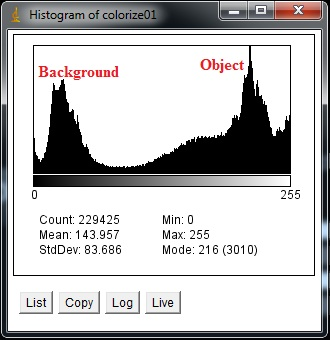
\includegraphics[width=1.00\textwidth]{Pictures/Theory/SimpleThresholdPicture} % Venstre billede
\end{minipage} \hfill
\begin{minipage}[b]{0.45\textwidth} \centering
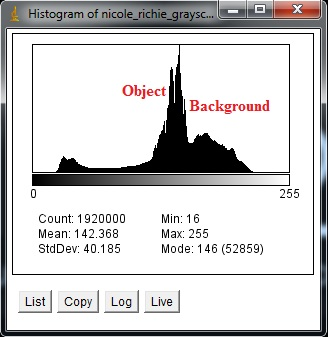
\includegraphics[width=1.00\textwidth]{Pictures/Theory/ComplicatedThresholdPicture} % Højre billede
\end{minipage} \\ % Captions og labels
\begin{minipage}[t]{0.45\textwidth}
\caption{Simple threshold value} % Venstre caption og label
\label{fig:SimpleThreshold}
\end{minipage} \hfill
\begin{minipage}[t]{0.45\textwidth}
\caption{Complicated threshold value} % Højre caption og label
\label{fig:ComplicatedThreshold}
\end{minipage}
\end{figure}

Looking at picture \eqref{fig:SimpleThresholdAfter} will show that the picture with the leftmost histogram, figure \eqref{fig:SimpleThreshold}, gives a clear outline of the silhouette of a woman after thresholding is applied. However, looking at figure \eqref{fig:ComplicatedThresholdAfter} shows that the picture with the rightmost histogram, figure \eqref{fig:ComplicatedThreshold}, gives a very poor silhouette of a woman because the background and the object has very similar colors. 

\begin{figure}[htbp] \centering
\begin{minipage}[b]{0.45\textwidth} \centering
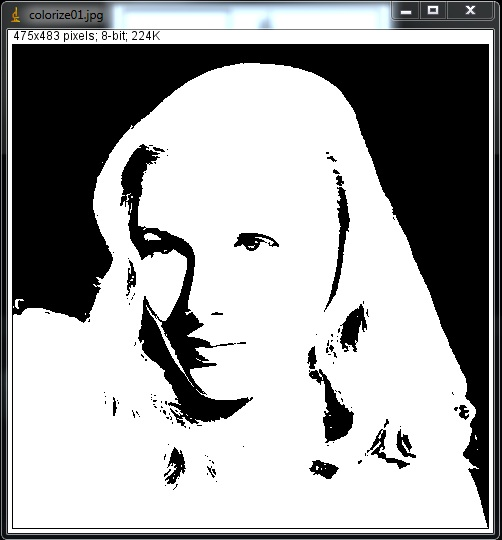
\includegraphics[width=1.00\textwidth]{Pictures/Theory/SimpleThresholdAfter} % Venstre billede
\end{minipage} \hfill
\begin{minipage}[b]{0.45\textwidth} \centering
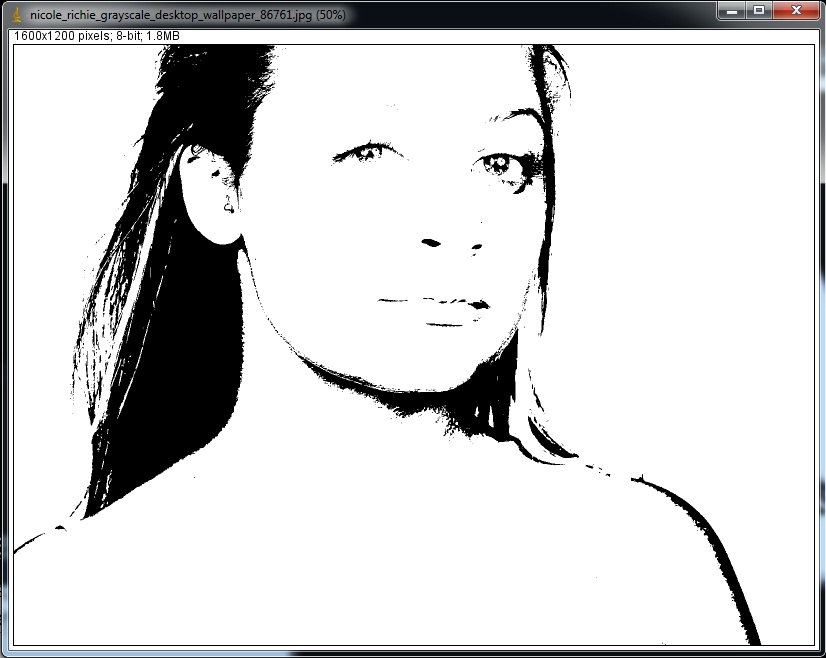
\includegraphics[width=1.00\textwidth]{Pictures/Theory/ComplicatedThresholdAfter} % Højre billede
\end{minipage} \\ % Captions og labels
\begin{minipage}[t]{0.45\textwidth}
\caption{Great silhouette after threshold} % Venstre caption og label
\label{fig:SimpleThresholdAfter}
\end{minipage} \hfill
\begin{minipage}[t]{0.45\textwidth}
\caption{Bad silhouette after threshold} % Højre caption og label
\label{fig:ComplicatedThresholdAfter}
\end{minipage}
\end{figure}
 
This proves the point that finding a functional threshold value is not always simple, and for finding a silhouette for example it is a great help to somehow make a clear transition from the object and the background.

\section{Morphology}
\subsection{Hit}
\subsection{Fit}
\subsection{Dilation}
\subsection{Erosion}
\subsection{Opening}
\section{BLOB-Analysis}
\section{Modified infrared camera vs normal webcam}
\section{Framework}
\section{Region of interest}
\section{Background subtraction}
\section{Template matching}
\section{movement tracking (ViBe)}
\section{Digital image}
\section{Noise filter(median/mean)}
A common problem when dealing with images is to determine if the image data contains a particular object or shape. The term BLOB stands for Binary Large Objects and refers to a region of connected pixels in a binary image. This technique is used to extract meaningful information from images and separate the pixels by detecting the points or regions that differ in properties like brightness or color changes (i.e., their value) and classifies them into two categories: the foreground (pixels with a non-zero value) and the background (pixels with a zero value).
Therefore, BLOB analysis will be split in three main steps: \textit{Extraction} of the BLOBs, \textit{representation} of the BLOBs and lastly, \textit{classification} of the BLOBs to know which ones belong to the expected type.
\subsection{BLOB Extraction}
To isolate BLOBs in a binary image, we need to define first if two pixels are connected or not. This is done by applying algorithms that will help to determine the connectivity of the pixels, but also the number of BLOBs contained in an image.
The most common used connectivities in BLOB extraction are the 8-connectivity and the 4-connectivity kernels. Whereas the 8-connectivity kernel is more accurate, it also requires more computations and consequently, needs more time to process the image.
\subsection{BLOB Classification}
The classification of the BLOBs is made by creating a \textit{prototype model} of the object that we are looking for, in order to state the features that it should accomplish, and the deviation that would be acceptable.

